\section{Основная часть}

\subsection{Первый подраздел}

\begin{definition}
    \textbf{Прямоугольник} --- это четырехугольник с прямыми углами.
\end{definition}

\begin{lemma}
    В прямоугольном треугольнике квадрат длины гипотенузы равен сумме квадратов длин катетов.
\end{lemma}
\proof
Для начала, обозначим катеты прямоугольного треугольника $a$ и $b$, а гипотенузу $c$. Тогда по теореме Пифагора:

\begin{equation}
    a^2 + b^2 = c^2
\end{equation}

Также, площадь прямоугольного треугольника равна половине площади прямоугольника со сторонами $a$ и $b$:

\begin{equation}
    S_{\triangle} = \frac{1}{2} ab
\end{equation}

Площадь же квадрата, по определению, равна квадрату длины его стороны, т.~е.~$c^2$.

Осталось доказать, что $c^2 = a^2 + b^2$. Для этого можно воспользоваться геометрическим доказательством, построив квадрат на каждом катете и увидев, что их площади в сумме равны площади квадрата на гипотенузе.

\begin{equation}
    \begin{tikzpicture}
        \newcommand{\pythagwidth}{3cm}
        \newcommand{\pythagheight}{2cm}

        \coordinate [label={below right:$A$}] (A) at (0, 0);
        \coordinate [label={above right:$B$}] (B) at (0, \pythagheight);
        \coordinate [label={below left:$C$}] (C) at (-\pythagwidth, 0);

        \coordinate (D1) at (-\pythagheight, \pythagheight + \pythagwidth);
        \coordinate (D2) at (-\pythagheight - \pythagwidth, \pythagwidth);

        \draw [very thick] (A) -- (C) -- (B) -- (A);

        \newcommand{\ranglesize}{0.3cm}
        \draw (A) -- ++ (0, \ranglesize) -- ++ (-\ranglesize, 0) -- ++ (0, -\ranglesize);

        \draw [dashed] (A) -- node [below] {$b$} ++ (-\pythagwidth, 0)
        -- node [right] {$b$} ++ (0, -\pythagwidth)
        -- node [above] {$b$} ++ (\pythagwidth, 0)
        -- node [left] {$b$} ++ (0, \pythagwidth);

        \draw [dashed] (A) -- node [right] {$a$} ++ (0, \pythagheight)
        -- node [below] {$a$} ++ (\pythagheight, 0)
        -- node [left] {$a$} ++ (0, -\pythagheight)
        -- node [above] {$a$} ++ (-\pythagheight, 0);

        \draw [dashed] (C) -- node [above left] {$c$} (B)
        -- node [below left] {$c$} (D1)
        -- node [below right] {$c$} (D2)
        -- node [above right] {$c$} (C);

    \end{tikzpicture}
\end{equation}

\begin{equation*}
    \begin{aligned}
        S_{\square ABC} & = \frac{1}{2} ab + \frac{1}{2} ab + \frac{1}{2} c^2 \
                        & = ab + \frac{1}{2} c^2 \
                        & = \frac{1}{2} c^2 + \frac{1}{2} c^2 \
                        & = c^2 \
    \end{aligned}
\end{equation*}

Таким образом, доказано, что $c^2 = a^2 + b^2$.
\lemp

\begin{theorem}[Пифагора]
    В прямоугольном треугольнике квадрат длины гипотенузы равен сумме квадратов длин катетов.
\end{theorem}
\proof
По лемме 1.
\thmp

\begin{figure}[h]
    \centering
    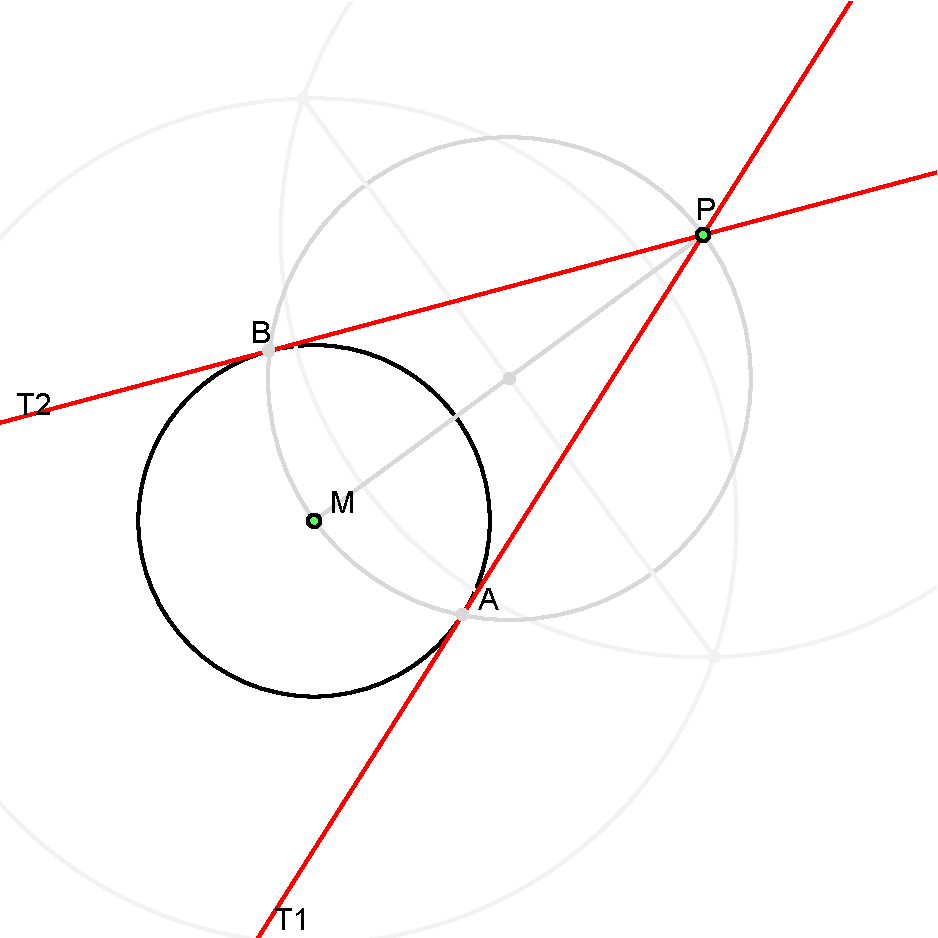
\includegraphics{math_geom_static_jsxgraph.pdf}
    \caption{Название рисунка}
\end{figure}


\subsection{Второй подраздел}

\begin{remark}
Не все прямоугольники являются квадратами.
\end{remark}

\begin{example}
Пример прямоугольника, который не является квадратом: прямоугольник со сторонами $3$ и $4$.
\end{example}

\begin{figure}[h]
    \centering
    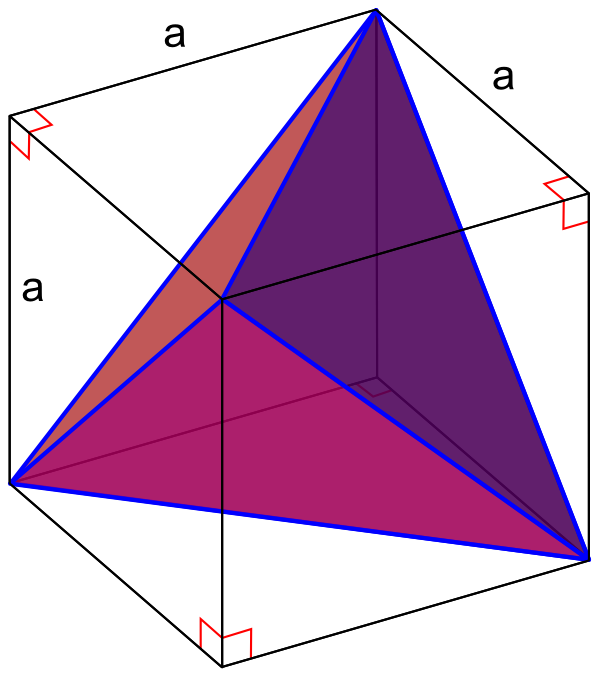
\includegraphics{regular_tetrahedron.png}
    \caption{Название рисунка}
\end{figure}